%!TEX root = ../template.tex
%%%%%%%%%%%%%%%%%%%%%%%%%%%%%%%%%%%%%%%%%%%%%%%%%%%%%%%%%%%%%%%%%%%
%% chapter1.tex
%% NOVA thesis document file
%%
%% Chapter with introduction
%%%%%%%%%%%%%%%%%%%%%%%%%%%%%%%%%%%%%%%%%%%%%%%%%%%%%%%%%%%%%%%%%%%

\typeout{NT FILE 02_sota.tex}%

\chapter{Research Context and State-of-the-Art}\label{cha:sota}

In this chapter, we outline the research context and review the
state-of-the-art in 3D scene understanding, with a focus on its application to
power grid inspection. Section~\ref{sec:3d_scene_understanding} introduces 3D
point clouds and reviews the main methodological approaches: projection-based,
voxel-based, point-based, and hybrid models. It also covers the role of
benchmarking datasets in driving model development.
%
Section~\ref{sec:inductive_biases} discusses inductive biases in 3D deep
learning, including the use of convolutional and group-equivariant operators,
and examines their strengths and limitations in handling irregular spatial
data. Section~\ref{sec:geneos} builds on this by exploring recent work on group
equivariant non-expansive operators and their potential for capturing
structural patterns in 3D scenes.
%
Lastly, Section~\ref{sec:3d_scene_understanding_power_grid} shifts focus to the
domain of power grid inspection. We review current manual
practices, survey available datasets and tools, and highlight the unique
challenges of deploying machine learning in this safety-critical, real-world
setting.

%-----------------------------
\section{Overview of 3D Scene Understanding}\label{sec:3d_scene_understanding}

This section provides an overview of 3D scene understanding methodologies,
classifying them based on their data representations and processing strategies.
These approaches include projection-based, voxel-based, point-based, and hybrid
methods. Each has its own strengths and limitations, particularly in handling
data sparsity, scalability, computational complexity, and generalization to
unseen environments.

Semantic segmentation aims to divide a 3D point cloud into subsets based on the
semantic meanings assigned to individual points. This process requires a
comprehensive understanding that simultaneously considers both the overarching
geometric structure and the fine-grained details of each point. According to
the taxonomy introduced by Guo et al.~\cite{guo2020deep}, semantic segmentation
methodologies are typically categorized into three main paradigms:
projection-based, discretization-based (voxel), and point-based methods. More
recently, hybrid approaches have emerged to leverage the advantages of each
individual class.

\subsection{Introducing 3D Point Clouds}

Point clouds have become a standard representation for capturing and analyzing
three-dimensional environments. At their core, point clouds are unordered sets
of points defined in Euclidean space, typically represented as $\mathcal{P} \in
    \mathbb{R}^{N \times (3 + F)}$, where $N$ is the number of points, each
described by spatial coordinates $(x, y, z)$ and $F$ are optional additional
features such as color (RGB), surface normals, intensity, or semantic labels.

The widespread adoption of depth-sensing technologies, such as LiDAR and RGB-D
cameras~\cite{alexiadis2014fast,song2016robust}, has facilitated the collection
of large-scale point cluds.
%
Consumer devices like smartphones and autonomous vehicles now routinely
generate high-resolution point clouds~\cite{li2020lidar}, fueling the creation
of large-scale annotated datasets such as ScanNet~\cite{dai2017scannet},
S3DIS~\cite{armeni20163d}, KITTI~\cite{behley2019semantickitti}, among others.
These resources have become foundational benchmarks for advancing 3D scene
understanding using data-driven approaches.

Even though point clouds have a compact format and are extremely detailed, they
also pose a unique set of challenges for deep learning methods, primarily due
to their irregular, unordered, and variable-density nature:

\textbf{Irregular Sampling and Heterogeneous Density:} Unlike images that
present uniform pixel spacing, point clouds may exhibit uneven sampling densities across different
parts of a scene. Objects can have both dense and sparse regions depending on
occlusions, sensor perspective, or reflectivity, as shown in Fig.~\ref{fig:pcd_props}~(a).
This irregularity complicates local feature extraction and challenges models
reliant on fixed-size neighborhoods (e.g., k-NN), which can either miss fine-grained details or
incorporate irrelevant context.

\textbf{Lack of Structure:} Point clouds are inherently unstructured.
They do not lie on a regular grid, and there is no implicit ordering or spatial
adjacency like in image pixels, as illustrated in Fig.~\ref{fig:pcd_props}~(b).
This absence of structure means that traditional convolutional architectures
are not directly applicable.
Instead, learning effective point-wise representations requires custom
aggregation functions or graph-based reasoning to capture local geometry
and long-range dependencies.

\textbf{Permutation Invariance:} Point clouds are independent of the order
in which they are stored, as it does not change the represented scene.
This is depicted Fig.~\ref{fig:pcd_props}~(c).
Deep learning methods often correlate the order of the input to the
intended output. However, invariance to permutations clashes with this
behavior. As a result, state-of-the-art methods often show additional
strategies to mitigate this challenge.

\begin{figure}[t]
    \centering
    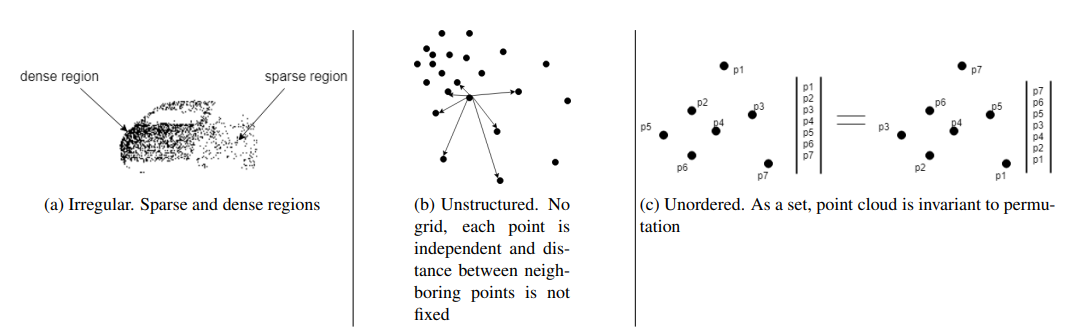
\includegraphics[width=1\linewidth]{sota_images/PCD_Props.png}
    \caption[Key challenges in processing 3D point clouds]
            {Key challenges in processing 3D point clouds~\cite{bello2020deep}.
        (a) Heterogeneous density: objects may contain both densely and sparsely sampled regions,
        complicating local feature extraction.
        (b) Lack of structure: unlike images, point clouds do not lie on a regular grid,
        requiring custom neighborhood and aggregation strategies.
        (c) Permutation invariance: the order of points does not alter the underlying geometry,
        demanding specialized model designs to ensure robustness.}\label{fig:pcd_props}
\end{figure}

\subsection{Projection-based Methods}
A straightforward strategy to apply well-established 2D learning techniques to
3D data is to project point clouds into multiple 2D views.
%
Projection-based methods render 3D scenes from different camera perspectives
and apply 2D convolutional neural networks (CNNs) to the resulting images,
typically RGB or depth maps. This paradigm benefits from leveraging powerful
pretrained 2D backbones, such as ResNet~\cite{he2015deep}, and has shown strong
performance in early 3D classification and retrieval
tasks~\cite{su2015multi,feng2018gvcnn,yang2019learning,lawin2017deep,lyu2020learning}.
%

Despite these strengths, the inherent loss of depth information and the
difficulty of occlusion handling limit their expressiveness in more complex
tasks. For instance, multi-view pipelines may struggle to accurately capture
spatial context or reconstruct fine 3D structures, which are essential for
scene-level tasks such as 3D semantic segmentation or object
detection~\cite{guo2020deep}.
%
Moreover, generating and fusing multiple 2D projections can introduce
additional computational overhead.
%
Consequently, projection-based methods have been mostly superseded by more
expressive volumetric or point-based approaches in current research.

\subsection{Voxel-based Methods}
To introduce structure into the inherently unstructured nature of point clouds,
voxel-based methods discretize 3D space into regular grids, typically denoted
as $N \times M \times K$ voxel volumes. Each voxel aggregates local geometric
information, often through occupancy or density statistics, allowing the use of
3D convolutional kernels over the structured tensor. Early works such as
VoxNet~\cite{maturana2015voxnet} and more recent advances like
MinkowskiNet~\cite{choy20194d} demonstrate the viability of this approach for
large-scale scene understanding.
%

However, voxelization comes with critical trade-offs. Coarse voxel grids
introduce spatial quantization errors and remove fine details of the geometry,
while finer grids lead to prohibitive memory consumption due to the cubic
growth of the voxel space and its inherent sparsity. High-resolution
voxel-based methods, such as OctNet~\cite{riegler2017octnet} and
O-CNN~\cite{wang2017cnn}, mitigate these issues by leveraging hierarchical
spatial structures (e.g., octrees) that selectively refine voxels only in
occupied regions. Nonetheless, 3D convolutions remain computationally more
expensive than their 2D counterparts (with a relative cost 3 times higher), 
making voxel-based methods less efficient for real-time applications.

\subsection{Point-based Methods}
Rather than altering the input structure, point-based methods operate directly
on raw point clouds without imposing a voxel grid or projecting the data. This
preserves the geometric fidelity of the original input and avoids quantization
artifacts. The seminal PointNet architecture~\cite{qi2017pointnet} pioneered
this idea by applying shared Multi-Layer Perceptrons (MLPs) to each point
individually, followed by a symmetric global aggregation function to ensure
permutation invariance.
%
Building on this, PointNet++~\cite{qi2017pointnet++} introduced hierarchical
feature learning by grouping points into local neighborhoods, enabling the
extraction of local geometric features.
%
Since then, a rich landscape of point-based methods has emerged, employing
point convolutions~\cite{thomas2019kpconv}, attention
mechanisms~\cite{zhao2021point}, or newer version of MLP-based
networks~\cite{qian2022pointnext} to better capture inter-point relationships.

Even though these approaches achieve state-of-the-art results across numerous
benchmarks, they are challenged with the unique challenges associated with
point clouds described above.
%
For instance, defining and processing local neighborhoods efficiently remains
challenging due to the non-uniform and sparse nature of point cloud data.

\subsection{Hybrid-based Methods}
Hybrid methods seek to unify the advantages of multiple representations by
fusing voxel-based, point-based, and sometimes image-based inputs into a single
framework. These models aim to overcome the limitations of individual paradigms
by leveraging structured representations for efficient computation while
retaining the geometric precision of raw
points~\cite{liu2019point,yan20222dpass,cheng20212,liu2023uniseg}.

Despite this, hybrid methods often come with increased architectural complexity
and require careful design to balance the contributions of each modality.
Additionally, they demand large-scale, diverse datasets and significantly
increased computational resources. These models often involve hundreds of
millions of parameters and require prolonged training on specialized hardware
setups.

\subsection{Benchmarking Datasets}

Benchmark datasets play a crucial role in the development and evaluation of 3D
deep learning methods. They offer standardized scenes and ground truth
annotations for tasks such as object classification, semantic segmentation,
part segmentation, and 3D object detection.
%

For indoor-scene mapping, datasets such as ScanNet~\cite{dai2017scannet} and
S3DIS~\cite{armeni20163d} are dominant. ScanNet provides over 1,500 RGB-D scans
of indoor environments with dense annotations for 20 object classes, captured
using a handheld RGB-D sensor. S3DIS, on the other hand, contains 3D scans of
six large-scale indoor areas, with detailed point-wise labels, making it
particularly useful for evaluating segmentation performance under clutter and
occlusion.

For outdoor large-scale segmentation, the benchmark of choice is
SemanticKITTI~\cite{behley2019semantickitti}, which offers point-wise labels
over full LiDAR sequences from the KITTI Odometry dataset. Captured with a
Velodyne HDL-64E sensor, it introduces challenges such as motion blur,
sparsity, and occlusions, pushing models to handle dynamic and noisy data.
Datasets like nuScenes~\cite{caesar2020nuscenes} and Waymo
Dataset~\cite{sun2020scalability} further extend these ideas by integrating
multimodal sensors (e.g., radar, camera) and offering annotations for 3D
detection and tracking across diverse driving scenarios.

In object part segmentation, datasets such as ShapeNet~\cite{chang2015shapenet}
and PartNet~\cite{mo2019partnet} have become the standard for part segmentation
over individual objects. ShapeNet provides over 16,000 3D models from 16
categories with point-wise part labels (e.g., airplane: wings, tail, engines),
and is widely used in benchmarking point-based networks. PartNet builds on this
by introducing hierarchical, instance-level part decompositions across
thousands of models, enabling the evaluation of both coarse and fine-grained
segmentation.

%-----------------------------
\section{Inductive Biases in 3D Deep Learning}\label{sec:inductive_biases}
% Discuss the broader role of inductive biases in ML, then focus on how geometric priors can guide 3D scene understanding.

This section details the role of inductive biases in deep learning, with an
emphasis on their impact in computer vision tasks. We begin by defining
inductive biases in the context of machine learning. We then review canonical
operators like convolution in 2D and 3D. Finally, we survey group equivariant
methods and assess the current landscape of successes and limitations in this
space.

\subsection{Understanding Inductive Biases}
% Define inductive bias in ML. Give classic 2D examples (e.g., translation equivariance in CNNs) and motivate why they matter in data-scarce or noisy regimes.

Inductive biases are the assumptions underlying a model's design that guide its
ability to generalize beyond the training data.
%
While machine learning frameworks aim to learn patterns directly from data, no
single learning algorithm can succeed at all possible tasks without constraints
or prior knowledge.
%
This is a consequence of the no-free-lunch
theorem~\cite{baxter2000model,goyal2022inductive}.
%
In high-dimensional or data-scarce regimes, inductive biases are essential to
guide learning and ensure generalization.

The success of convolutional neural networks in 2D vision tasks stems not from
increased expressiveness, after all, multi-layer perceptrons are universal
function approximators, but from their architectural inductive biases.
%
CNNs exploit local correlations and embed translation equivariance directly
into the feature extraction process. These assumptions yield better parameter
efficiency, generalization, and interpretability, especially when data is
limited or noisy.

In 3D scene understanding, the challenge is more severe.
%
Point clouds lack a regular structure, they show variations in scale,
orientation, and sparsity, all of which complicate direct application of 2D
priors.
%
Thus, we propose geometric inductive biases, rooted in spatial and topological
properties of 3D data, for learning meaningful representations of such data.

\subsection{The Convolution Operator}
% Review the adaptations of convolution for 3D. Cover both spatial and graph-based operators.

The convolution operator has been a foundational tool in deep learning,
particularly in computer vision, due to its locality, parameter sharing, and
equivariance properties.

\subsubsection{Theoretical Formulation}

At its core, convolution is a mathematical operation that blends two functions
by integrating their product over space.
%
This effectively measures the similarity between a signal (e.g., an image) and
a filter.
%
The continuous convolution operator between an input function $f(x)$ and a
kernel $g(x)$ is defined as:

\begin{equation}\label{eq:theo-conv}
    (f * g)(x) = \int_{\mathbb{R}^n} f(t) \cdot g(x - t) dt.
\end{equation}

In the context of deep learning, this operation is discretized and implemented
as a series of matrix multiplications.
%
In image processing (typically $n = 2$), $f$ represents the image and $g$ is
the convolutional kernel.
%
The kernel is shifted across the domain of the input, producing a response at
each location.
%
In discrete 2D convolution, the continuous convolution in~\eqref{eq:theo-conv}
is approximated by a discrete sums. For an image $I \in \mathbb{R}^{H \times W
        \times C}$ and a kernel $K \in \mathbb{R}^{k \times k \times C}$, the operation
becomes:

\begin{equation}\label{eq:discrete-conv}
    (I * K)[i, j] = \sum_{m}^{k-1} \sum_{n}^{k-1} I[i + m, j + n] \cdot K[m,n].
\end{equation}

This sums over a local neighborhood centered at pixel $[i, j]$, producing an
output that emphasizes certain features, such as edges or textures, depending
on the kernel's learned weights.

\subsubsection{Extension to 3D Point Clouds}

The lack of structure and irregular density in point clouds sharply contrasts
with the regular grid structure of images.
%
To address this, projection-based and voxel-based methods force point clouds
into a structured grid, allowing 2D and 3D CNNs methods to be employed.
%
The convolution operator extends naturally to 3D tensors:

\begin{equation}\label{eq:3d-discrete-conv}
    (I * K)[i, j, k] = \sum_{m}^{k-1} \sum_{n}^{k-1} \sum_{p}^{k-1} I[i + m, j + n, k + p] \cdot K[m,n,p].
\end{equation}

This 3D convolution operates over a cubic neighborhood and is used in models
that take voxelized inputs. Due to the cubic growth of the input space, 3D
convolutions are computationally expensive and memory-intensive, especially for
high-resolution data.
%

To effectively apply convolutions to point clouds, the convolution operator
must be adapted to work with their irregular sampling and lack of grid
structure.
%
To this end, point-based methods have introduced several strategies that
interpret point clouds as geometric graphs, where each point is a node and
edges are defined based on local
neighborhoods~\cite{hermosilla2018monte,simonovsky2017dynamic}.
%
These methods are divided by the nature of their convolution kernels:
%
discrete-kernel
methods~\cite{lei2019octree,thomas2019kpconv,lei2020spherical,zhu2021cylindrical,wang2019graph}
follow standard CNN kernels and define filters in euclidean space, similar to
3D-CNN kernels for voxel-grids~\cite{maturana2015voxnet}.
%
For example, KPConv~\cite{thomas2019kpconv} employs a point-convolution where
the kernel is defined as a set of $K$ points in 3D space, each with a weight
that is learned during training. The convolution operation is then performed by
computing the weighted sum of the features of the neighboring points within a
certain radius.
%
In turn, continuous-kernel
methods~\cite{groh2018flex,wang2018deep,xu2018spidercnn,li2018pointcnn,wu2019pointconv}
take a more flexible approach by learning the convolution weights as a function
of the relative positions between points. A common formulation is: $w_{ij} =
    h(x_j - x_i)$, where $x_i$ is the center point, $x_j$ one of its neighbors, and
$h$ is a learnable funtion, often implemented as a multi-layer perceptron
(MLP).
%
This design allows the network to dynamically adapt the convolution filter to
the local geometry, rather than relying on a fixed grid.
%

\subsection{Group Equivariant Methodologies}
% Discuss works that explicitly build equivariant architectures (e.g., Tensor Field Networks, SE(3)-Transformers, EGNN). 

3D scene understanding often entails reasoning about objects that appear in arbitrary
orientations and positions. This poses a challenge for traditional models
because they are typically sensitive to such transformations unless explicitly
trained to account for them.
%
A possible approach to overcome this limitation is the incorporation of group
equivariance into neural networks.
% This concept, rooted in group theory,
% allows models to learn representations that are invariant to specific transformations,
% such as rotations and translations, by leveraging the underlying symmetries of the data.

Equivariance is a property of a function or an operator that preserves the structure of the
input space under a specific group of transformations.
%
Formally, an operator $f: \mathcal{X} \rightarrow \mathcal{Y}$ is said to be
\emph{equivariant} with respect to a group of transformations $G$ if for every
transformation $g \in G$, the following holds:
\begin{equation}\label{eq:equivariance}
    f(g \cdot x) = \rho(g) \cdot f(x), \quad \forall x \in \mathcal{X},
\end{equation}
%
where $g \cdot x$ denotes the action of $g$ on the input $x$, and $\rho(g)$ is
a (possibly different) representation of $g$ acting on the output space
$\mathcal{Y}$.
%
For example, consider standard 2D convolutions in image processing. These are
translation-equivariant, meaning that if the input image is shifted in space,
the resulting feature maps the shift in the same way:
\begin{equation}\label{eq:translation-equivariance}
    \text{Conv}(T_{\Delta x} x) = T_{\Delta x}(\text{Conv}(x)),
\end{equation}
where $T_{\Delta x}$ denotes a translation by $\Delta x$.

In 3D scene understanding, transformations of interest include translations,
rotations and reflections, typically represented by the Euclidean group E(n) or
the special Euclidean group SE(n).
%
Designing models that are equivariant to such groups allows them to reason
about objects and structures in a way that mirrors the physical symmetries of
the world. This means, for instance, that rotating a 3D object in space will
result in a corresponding, interpretable rotation of the model’s internal
features, rather than forcing the network to learn the rotation through
brute-force data augmentation.
%

Recent advances in geometric deep learning have introduced explicitly
equivariant architectures that enforce equivariance through their network
design.
%
These models typically employ specialized layers that are equivariant to
rotations and translations, allowing them to learn representations that are
invariant to these transformations.
%
G-convolutions~\cite{cohen2016group} generalize the conventional
translation-equivariant convolution to arbitrary groups. However, in practice,
they are often limited to small groups like \textit{p4} group, incorporating
transla- tions and 90-degree rotations, and the \textit{p4m} group, which also
includes reflections.
%
Tensor Field Networks (TFN)~\cite{thomas2018tensor} uses tensor fields to
represent the input data and incorporates rotationally equivariant operations
to process these tensors.
%
SE(3)-Transformers~\cite{fuchs2020se} extend the attention mechanism to be
equivariant to rotations and translations, enabling the model to learn
relationships between points in a way that respects the symmetries of the data.
%
Graph Neural Networks (GNN)~\cite{satorras2021n}, on the other hand, employ a
graph-based approach to learn equivariant representations by iteratively
updating node features based on local neighborhoods, ensuring that the updates
are equivariant to rotations and translations.

\subsection{Effectiveness and Limitations}
Inductive biases, when carefully chosen and implemented, can lead to
substantial gains in performance, generalization, and interpretability.
%
However, limitations remain. First, designing equivariant architectures often
involves a trade-off between expressiveness and computational cost. Second,
while group equivariant methods generalize well to known transformations, they
may struggle when the data distribution violates assumed symmetries. Third,
explicit priors can constrain learning if they misalign with the task, and
tuning such priors requires domain expertise.
%
Moreover, despite growing interest, the field lacks standardized benchmarks to
evaluate the contribution of inductive biases across diverse 3D tasks.

\section{Group Equivariant Non-expansive Operators}\label{sec:geneos}

Group Equivariant Non-Expansive Operators (GENEOs) offer a mathematically
grounded framework for incorporating geometric priors and equivariant behavior
into learning models. Introduced by Bergomi et al.~\cite{bergomi2019towards}
and later extended in subsequent
works~\cite{cascarano2021geometric,conti2022construction}, this framework views
machine learning agents not merely as parameterized functions, but as operators
acting on spaces of functions that represent data.
%
GENEOs extract essential features from the data, similar to how CNN kernels
identify important patterns to recognize objects. These agents, or observers,
transform data into higher-level representations while adhering to a set of
properties defined by a group of transformations. An effective observer
transforms data in a way that commutes with these transformations, making it
equivariant with respect to the transformation group.

At the heart of the GENEO formalism lies the concept of a \emph{perception
    pair}, denoted by $(\Phi, G)$. Here, $\Phi$ is a set of real-valued functions
defined over a domain $X$, i.e., $\phi: X \rightarrow \mathbb{R}$, representing
the admissible observations or measurements on the domain.
%
For example, a grayscale image can be interpreted as a function assigning
intensity values to each pixel location, while a 3D point cloud may be encoded
as a function describing density or occupancy across space.
%
By representing data in this functional form, GENEOs shift the focus from raw
data points to the space of measurements, allowing for a more abstract and
general treatment of geometric structure.
%
The group $G$ encodes the symmetries or transformations under which the data is
assumed to vary, such as translations, rotations, or more general isometries.
Crucially, it is assumed that this group acts on $\Phi$ via function
composition: for any transformation $g \in G$ and any function $\phi \in \Phi$,
the transformed function $\phi \circ g$ must also lie within $\Phi$. This
requirement ensures that the space $\Phi$ is closed with respect to $G$,
and enables us to encode prior knowledge about data invariances or
equivariances directly into the functional representation.

\begin{definition}[Group Equivariant Non-Expansive Operator]
    Let $(\Phi, G)$ and $(\Psi, H)$ be two perception pairs,
    and let $T: G \rightarrow H$ be a group homomorphism.
    A map $F: \Phi \rightarrow \Psi$ is called a
    \emph{Group Equivariant Non-Expansive Operator} (GENEO)
    if it satisfies the following two properties:\\
    \textbf{Equivariance:}
    \begin{equation}
        F(\phi \circ g) = F(\phi) \circ T(g), \quad \forall g \in G, \forall \phi \in \Phi,
    \end{equation}
    and \textbf{Non-expansivity:}
    \begin{equation}
        \|F(\phi_1) - F(\phi_2)\|_\infty \leq \|\phi_1 - \phi_2\|_\infty, \quad \forall \phi_1, \phi_2 \in \Phi.
    \end{equation}

\end{definition}

GENEOs provide a rigorous way to define learning models that are both robust to
transformations and stable to small perturbations. From a topological
standpoint, the use of the $L_\infty$ norm induces a natural topology on $\Phi$
and $\Psi$, allowing the spaces of functions to be treated as compact metric
spaces under reasonable conditions.

Non-expansivity and convexity are essential for the applicability of GENEOs in
machine learning. When $\Phi$ and $\Psi$ are compact spaces, non-expansivity
guarantees that the set of all GENEOs is also compact. This compactness ensures
that any GENEO can be approximated by linear combination of a finite number of 
other GENEOs within the same space. 
%
Moreover, if $\Psi$ is convex, then the set of GENEOs is also
convex~\cite{bergomi2019towards}, meaning that convex combinations of GENEOs
yield new valid GENEOs. Together, these properties allow the construction of
efficient and expressive models through a finite and combinable basis of
operators.

In practice, these properties enable strong generalization with fewer
parameters, making GENEO-based models especially suitable for scenarios where
robustness to transformations and interpretability are critical. Applications
of GENEOs have been demonstrated in areas such as topological representation
learning~\cite{bergomi2019towards}, parameter-efficient
networks~\cite{bocchi2023finite}, and equivariant modeling for biomedical
imaging and 3D shape analysis~\cite{bocchi2022geneonet}.

\section{3D Scene Understanding for Power Grid Inspection}\label{sec:3d_scene_understanding_power_grid}

\subsection{Manual and Automated Inspection Practices}
%
Traditional inspection methods in power grid maintenance, such as ground
patrols and helicopter-based surveys, have been the industry standard for
decades. While effective, these approaches are costly, time-consuming, and
often limited by environmental conditions and human error. As power grids
expand into more remote and complex terrains, the limitations of these
practices have become increasingly evident.
%
Recent advancements in UAV (Unmanned Aerial Vehicle) technology, combined with
high-resolution LiDAR sensors, have enabled remote acquisition of dense 3D
point cloud data, offering a more scalable and efficient alternative. However,
despite the reduced need for on-site personnel during data collection, the
downstream processing and annotation of 3D scans remain largely manual. These
manual workflows are both labor-intensive and error-prone, particularly given
the volume and complexity of the data. To address these inefficiencies,
researchers have begun integrating 3D computer vision methods, particularly
semantic segmentation and object detection, into inspection pipelines. These
methods show promise in automatically identifying key elements such as power
lines, towers, and vegetation, thereby improving inspection throughput and
safety.

\subsection{Existing Datasets and Tools}

Progress in 3D scene understanding has been largely driven by high-quality
benchmark datasets. Most publicly available datasets, however, are geared
toward autonomous driving (e.g., KITTI~\cite{behley2019semantickitti},
nuScenes~\cite{caesar2020nuscenes}), indoor environments (e.g.,
ScanNet~\cite{dai2017scannet}, S3DIS~\cite{armeni20163d}), or synthetic 3D
object classification (e.g., ShapeNet~\cite{chang2015shapenet},
PartNet~\cite{mo2019partnet}). These datasets predominantly feature urban or
controlled environments and fail to represent the challenges inherent to rural
or utility-based inspection tasks.

To date, there are no publicly available datasets specifically tailored to
rural power grid systems. Some existing datasets include elements that are
tangentially relevant, but each presents critical limitations for this domain.
Forest3D~\cite{trochta20173d}, for example, is focused exclusively on tree
segmentation and instance-level forestry analysis, with no representation of
infrastructure. GTASynth~\cite{curnis2022gtasynth} simulates non-urban terrain
but is synthetic in nature and designed from a vehicle-mounted perspective,
resulting in low point densities and frequent occlusions.
NEON~\cite{marconi2019data} provides airborne LiDAR data with a focus on
vegetation and tree crown modeling, but does not include power grid
infrastructure.
%
DALES~\cite{varney2020dales} is among the few datasets to feature transmission
structures, but it is limited to high-voltage towers in urban environments.
High-voltage towers, due to their size and standardized geometry, are typically
unobstructed and relatively easy to detect. In contrast, medium- and
small-voltage towers exhibit diverse shapes and sizes and are frequently
occluded by vegetation or embedded within complex natural terrain, making it
significantly more challenging to identify and inspect.
%

Thus, there is a notable gap in publicly available datasets that adequately
capture the structural, environmental, and operational complexities of rural
power grid systems. A dataset that provides high-density, UAV-acquired 3D point
clouds of such environments would serve as a crucial benchmark for advancing
both semantic segmentation and object detection methods in this domain, and
enable the development of machine learning tools specifically tailored to power
grid inspection.

\subsection{Domain-specific Challenges}

Applying machine learning to power grid inspection introduces a set of
challenges that go beyond traditional model development or academic benchmarks.
In this domain, the stakes are high: \textbf{false negatives} can result in
undetected infrastructure failures, vegetation encroachment, or safety hazards,
while \textbf{false positives} can trigger unnecessary fieldwork, diverting
limited maintenance resources. As such, the threshold for reliability is
substantially higher than in many other 3D scene understanding applications.

One of the primary barriers to adoption is trust. Inspection tasks often
support critical decision-making, and utility providers require systems that
are not only accurate, but also explainable and robust under varying
conditions. This is particularly difficult in power grid environments, which
are characterized by highly variable structure types (e.g., differing tower
geometries), natural occlusions (e.g., trees, terrain), and sensor artifacts
introduced by weather or vegetation. A model must demonstrate consistent
performance across this diversity before it can be considered for integration
into operational workflows.
%
Additionally, class imbalance is a critical issue. Power lines and towers often
comprise a small fraction of the data collected during UAV inspections. Machine
learning models tend to overfit to dominant background classes such as ground
or vegetation. In the absence of mechanisms to handle class imbalance, model
predictions will fail to meet the precision and recall levels required for
risk-sensitive environments.

Operational integration presents another layer of complexity. For machine
learning to add value in this space, it must complement existing tools and
procedures. For instance, Geographic Information Systems (GIS), asset
management software, or human-in-the-loop validation protocols. This means that
ML models must produce interpretable outputs, offer confidence measures or
uncertainty estimates, and scale to large datasets acquired across thousands of
kilometers of transmission lines.

In short, deploying machine learning in power grid inspection is not only a
technical challenge, but an operational one. Success depends on building models
that are robust, interpretable, and able to meet the reliability standards
required in high-risk, safety-critical settings. Bridging this gap requires not
only improved algorithms and training data, but also thoughtful design of the
end-to-end inspection pipeline in which such models are deployed.

